% Compiled once while building the image so the packages and fonts a typical
% paper uses are already in the Tectonic cache. With the compile sandbox on,
% compiles cannot add to that cache, so anything used here is what documents
% can use. Add \usepackage lines to make more packages available.
\documentclass[11pt]{article}

\usepackage[english]{babel}
\usepackage{geometry}
\usepackage{amsmath, amssymb, amsthm, mathtools}
\usepackage{graphicx}
\usepackage{xcolor}
\usepackage{booktabs, tabularx, multirow, longtable, array}
\usepackage{caption, subcaption, float}
\usepackage{enumitem}
\usepackage{fancyhdr}
\usepackage{listings}
\usepackage{algorithm, algpseudocode}
\usepackage{siunitx}
\usepackage{tikz}
\usetikzlibrary{arrows.meta, positioning, shapes, calc}
\usepackage{pgfplots}
\pgfplotsset{compat=1.16}
\usepackage{csquotes}
\usepackage{microtype}
\usepackage{url}
\usepackage[numbers]{natbib}
\usepackage{hyperref}
\usepackage{cleveref}

\pagestyle{fancy}
\newtheorem{theorem}{Theorem}

\title{Cache Warm-up}
\author{poly-txt}
\date{}

\begin{document}
\maketitle

\begin{abstract}
Regular, \textbf{bold}, \textit{italic}, \textbf{\textit{bold italic}}, \textsc{Small Caps},
\texttt{monospace}, \textsf{sans serif}, and \enquote{quoted} text.
\end{abstract}

\section{Mathematics}\label{sec:math}
\begin{theorem}
For all $x \in \mathbb{R}$, $e^{i\pi} + 1 = 0$ and $\sum_{k=1}^{n} k = \frac{n(n+1)}{2}$.
\end{theorem}
\begin{proof}
See \cref{sec:math}, \cite{knuth}, and \url{https://example.com}.
\end{proof}
\begin{align}
  \mathcal{L}(\theta) &= \int_{-\infty}^{\infty} \lVert f(x) - \hat{f}_\theta(x) \rVert^2 \, dx
  \leq \mathfrak{A} \cdot \mathbf{v} \circledast \boldsymbol{\alpha}
\end{align}
A measurement of \SI{9.81}{\metre\per\second\squared}.

\section{Tables and Lists}
\begin{table}[H]
  \centering
  \begin{tabularx}{0.6\textwidth}{lX}
    \toprule
    \multirow{2}{*}{Key} & Value \\
    & \textcolor{blue}{Colored} \\
    \bottomrule
  \end{tabularx}
  \caption{A table.}
\end{table}
\begin{enumerate}[label=(\alph*)]
  \item First
  \item Second
\end{enumerate}

\section{Figures}
\begin{figure}[H]
  \centering
  \begin{subfigure}{0.45\textwidth}
    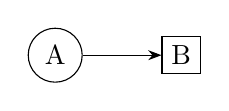
\begin{tikzpicture}
      \node[draw, circle] (a) {A};
      \node[draw, rectangle, right=of a] (b) {B};
      \draw[-Stealth] (a) -- (b);
    \end{tikzpicture}
    \caption{TikZ}
  \end{subfigure}
  \begin{subfigure}{0.45\textwidth}
    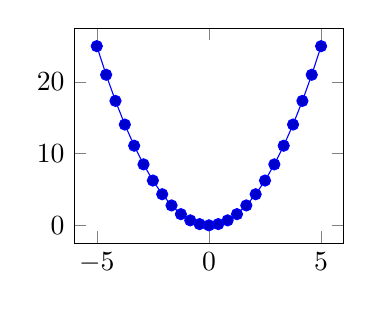
\begin{tikzpicture}
      \begin{axis}[width=5cm]
        \addplot {x^2};
      \end{axis}
    \end{tikzpicture}
    \caption{PGFPlots}
  \end{subfigure}
  \caption{Figures.}
\end{figure}

\section{Code}
\begin{lstlisting}[language=Python]
def add(a, b):
    return a + b
\end{lstlisting}
\begin{algorithm}[H]
  \caption{Algorithm}
  \begin{algorithmic}[1]
    \State $x \gets 0$
    \For{$i = 1$ to $n$} \State $x \gets x + i$ \EndFor
  \end{algorithmic}
\end{algorithm}

\bibliographystyle{plainnat}
\bibliography{references}
\end{document}
